% !TeX root = sigqdyn_tr.tex
% ================================================================
\section{Marking Fairness Experiments}\label{sec:marking_fairness_expts}\label{sec:marking_fairness_discuss}

% ----------------------------------------------------------------
\subsection{EST-based Marking Fairness}\label{sec:marking_fairness_expts_est}

\begin{figure*}[t!]
	\centering
	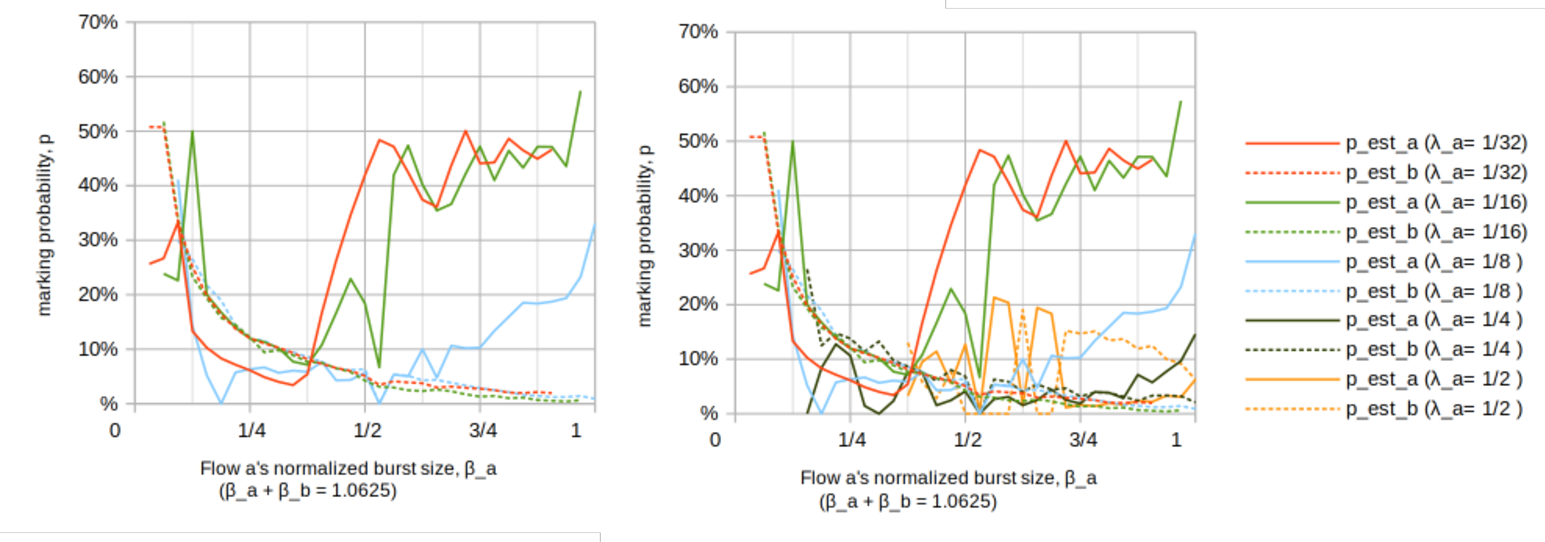
\includegraphics[width=\linewidth]{est-fairnessSumBeta10625}
	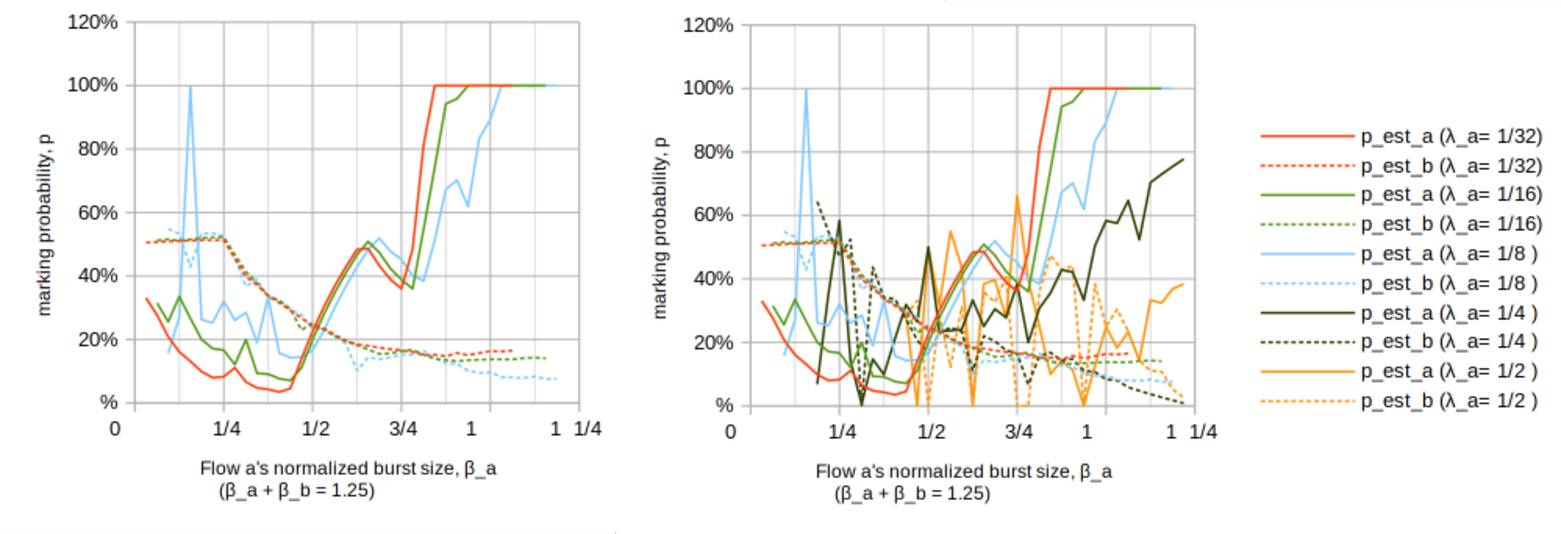
\includegraphics[width=\linewidth]{est-fairnessSumBeta125}
	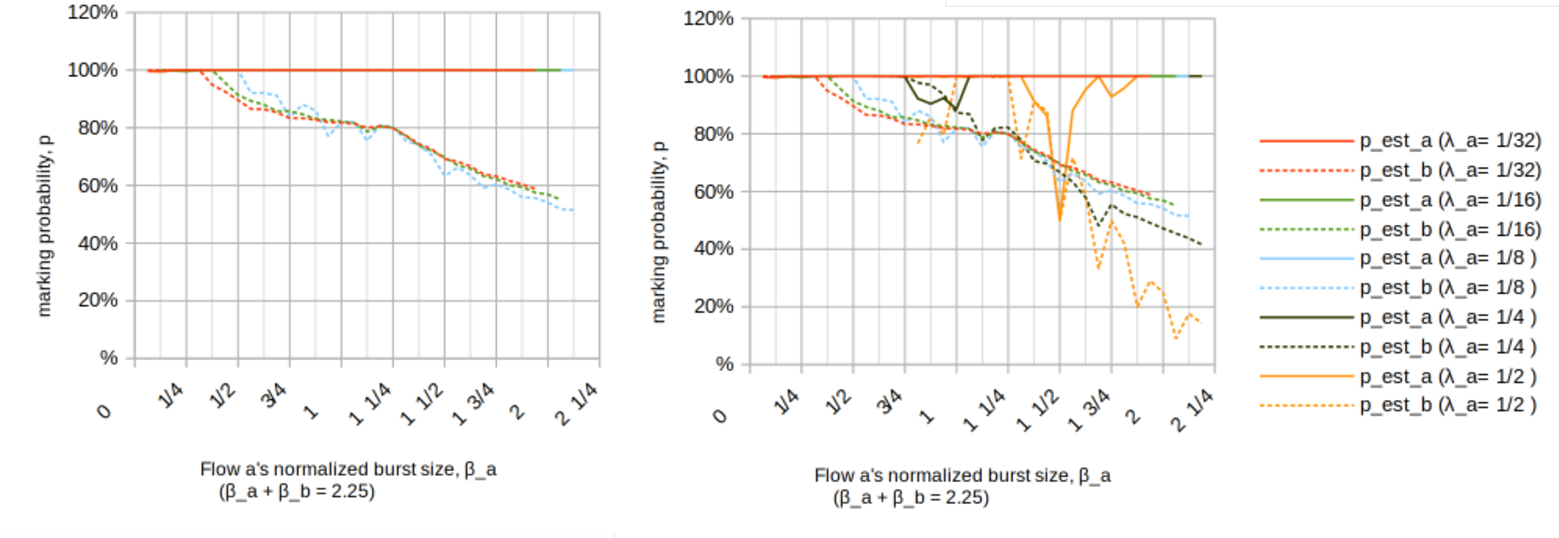
\includegraphics[width=\linewidth]{est-fairnessSumBeta225}
	\caption{EST-based marking fairness of two flows wrt capacity share, \(\lambda\), and relative burstiness of flow \(a, \beta_a\).\\
	\(\sum\lambda=100\%; \enspace\sum\beta=1.0625, 1.25, 2.25 \mathrm{(top, middle, bottom)}\). 
	The left-hand charts are the same as the right, except they exclude two scenarios that otherwise obscure the other plots}\label{fig:est-fairness-range}
\end{figure*}

\autoref{fig:est-fairness-range} shows the degree to which EST-based ECN marking is or is not focused onto the more bursty of a pair of flows indexed as \(a\) \& \(b\). Both flows were modelled as unresponsive in a time-slotted model similar to the example in \autoref{fig:marking-fairness5050}b). So the results are not necessarily an accurate reflection of a real AQM, but they should at least be indicative of the likely outcome.

The charts show the ECN marking level that results from scanning the scenario parameters across two dimensions:
\begin{enumerate}
	\item The capacity share of flow \(a\), \(\lambda_a\) is varied from \sfrac{1}{32} to \sfrac{1}{2} and the share the other flow \(b\) is also varied so that it fills the remainder of the link (\(\lambda_a+\lambda_b=100\%\))). The left-hand chart of each pair is identical to the right-hand chart except, to help pick out the plots, the last two capacity-share scenarios are omitted.
	\item The normalized burst size of flow \(a\), \(\beta_a\) is increased from \sfrac{1}{16} in steps of \sfrac{1}{16}, while the burst size of flow \(b\) is reduced such that the sum of both burst sizes is constant. Normalization is relative to the ECN marking threshold, so a sum of 1.25 means that if bursts from both flows coincide, a previously empty queue would exceed the marking threshold by 25\%. The sum increases from 1.0625 in the top plots, through 1.25 in the middle to 2.25 at the bottom, increasingly the likelihood of exceeding the threshold because a burst from one flow will not have drained enough when a burst from the other arrives.
\end{enumerate}

Bear in mind that, the average capacity share \(\lambda\) of each differently styled plot stays constant. So, as the burst size of flow \(a\) increases to the right its larger bursts have to become less frequent. And the burst size of flow \(b\) decreases to the right, so its smaller bursts become more frequent.

It can be seen from the right-hand side of any of the plots that, if flow \(a\) utilizes a small fraction of the capacity (up to roughly \sfrac{1}{8}) and if it is even slightly more bursty than the flow \(b\) (which is using more of the capacity), EST-based marking focuses a high fraction of the marking onto the more bursty flow. 

\begin{figure*}
	\centering
	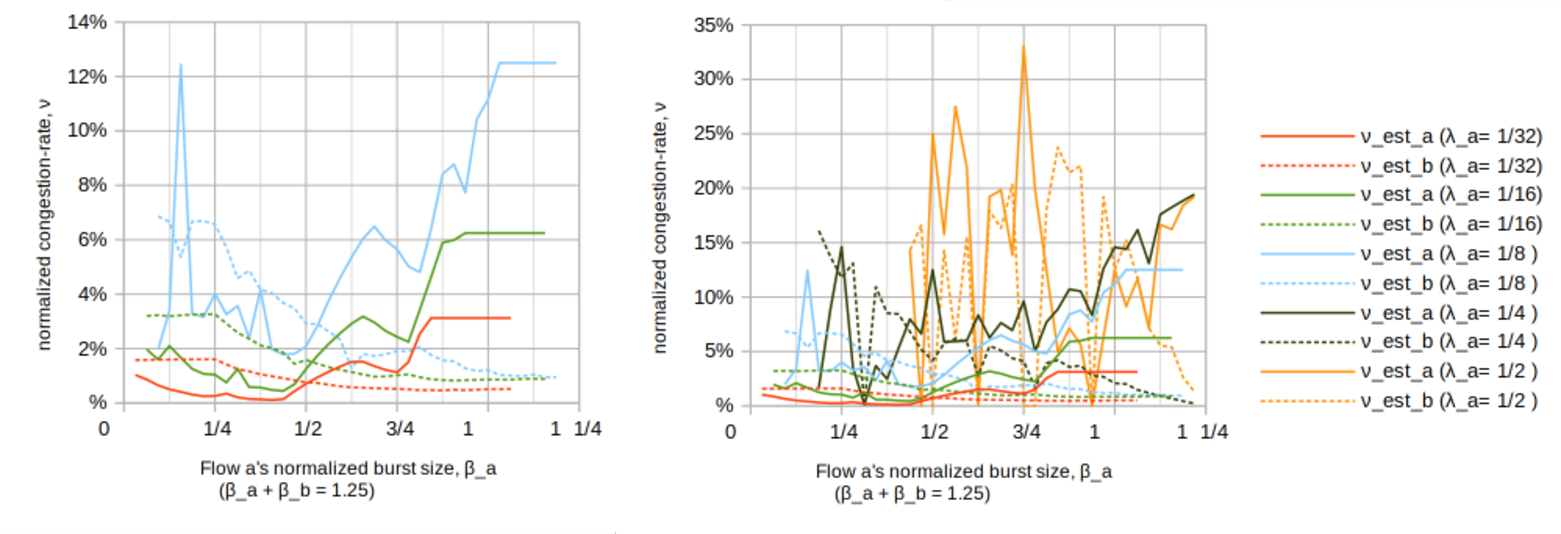
\includegraphics[width=\linewidth]{est-cong-rateSumBeta125}
	\caption{EST-based congestion-rate of two flows wrt capacity share, \(\lambda\), and relative burstiness, \(\beta\).\\
		\(\sum\lambda=100\%; \quad \sum\beta=1.25\) (same as middle row of \autoref{fig:est-fairness-range}). 
		The left-hand charts are the same as the right, except they exclude two scenarios that otherwise obscure the other plots}\label{fig:cong-rate-range}
\end{figure*}

It is also noticeable that wobbles increasingly appear; some so great that at certain points, even when sharing capacity 50:50, the more bursty flow attracts \emph{less} of the marking. It is possible that these wobbles are an artefact of the time-slotting in the model, so a more precise simulation will be necessary.

Working down from top to bottom of \autoref{fig:est-fairness-range}, it can also be seen that, as the combined level of burstiness increases, it pushes the marking level of the more bursty flow up to 100\% over a wider range of capacity shares, ultimately remaining at 100\% across any share of burstiness.

However, it must be admitted that the region where the plots of flow \(a\) and \(b\) cross (for any capacity share, \(\lambda_a\)) is always to the left of centre. The capacity share of \(a\) is never more than half, so this means that there is a range to the left of centre where \(a\)'s marking probability is higher even though both its burstiness and capacity share are lower than \(b\)'s, although this inversion corrects itself as \(b\)'s relative burstiness increases.

Focusing again on the right hand side of the charts (where flow \(a\) is more bursty than \(b\)), it may seem counter-intuitive that those flows with a smaller share of the capacity attract a higher marking probability. Even though \(a\)'s marking probability is still generally higher than \(b\)'s, the difference continually narrows, even where \(a\) is considerably more bursty than \(b\).

The explanation is that, when the size of flow \(a\)'s bursts relative to \(b\)'s remains the same (on the same vertical), but its share of capacity increases, its bursts will become more closely spaced. Then, they are more likely to arrive behind some of \(b\)'s traffic. So flow \(a\)'s marking probability will decrease as its capacity share increases.

Also it should be kept in mind that two flows with the same burstiness (on the vertical line down the middle of the plots) would be expected to have the same marking \emph{probability} even if they have different shares of capacity. But a flow with a lesser share of the capacity will attract a proportionately lesser share of the \emph{volume} of marks. This is explained in \autoref{fig:cong-rate-range}, which shows the same traffic scenario as the middle of \autoref{fig:est-fairness-range}, but the metric on the y-axis is normalized congestion-rate, which represents the proportion of link throughput that is marked, rather than just the proportion of flow \(a\). Or formally, the normalized congestion rate of flow \(a\), \(\nu_a = \lambda_a p_a\). With this metric it can be seen that, for the same relative burstiness (same vertical), the proportion of marks increases with capacity share, as would be expected intuitively.

\begin{figure*}
	\centering
	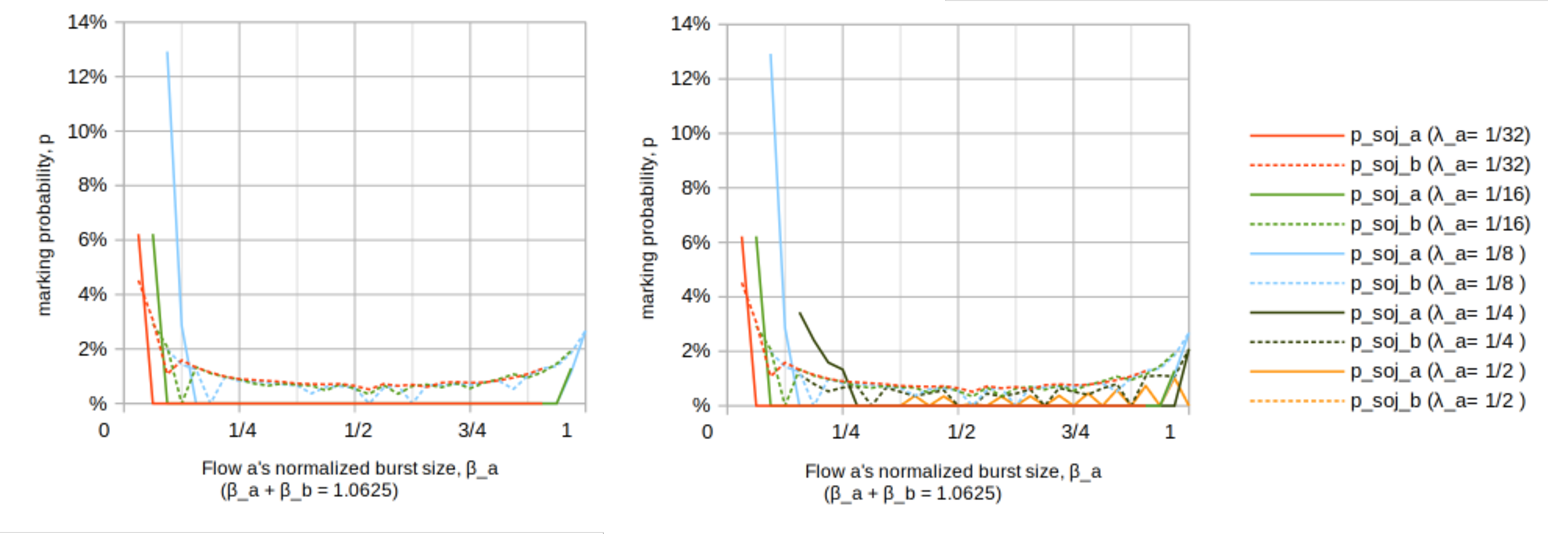
\includegraphics[width=\linewidth]{soj-fairnessSumBeta10625}
	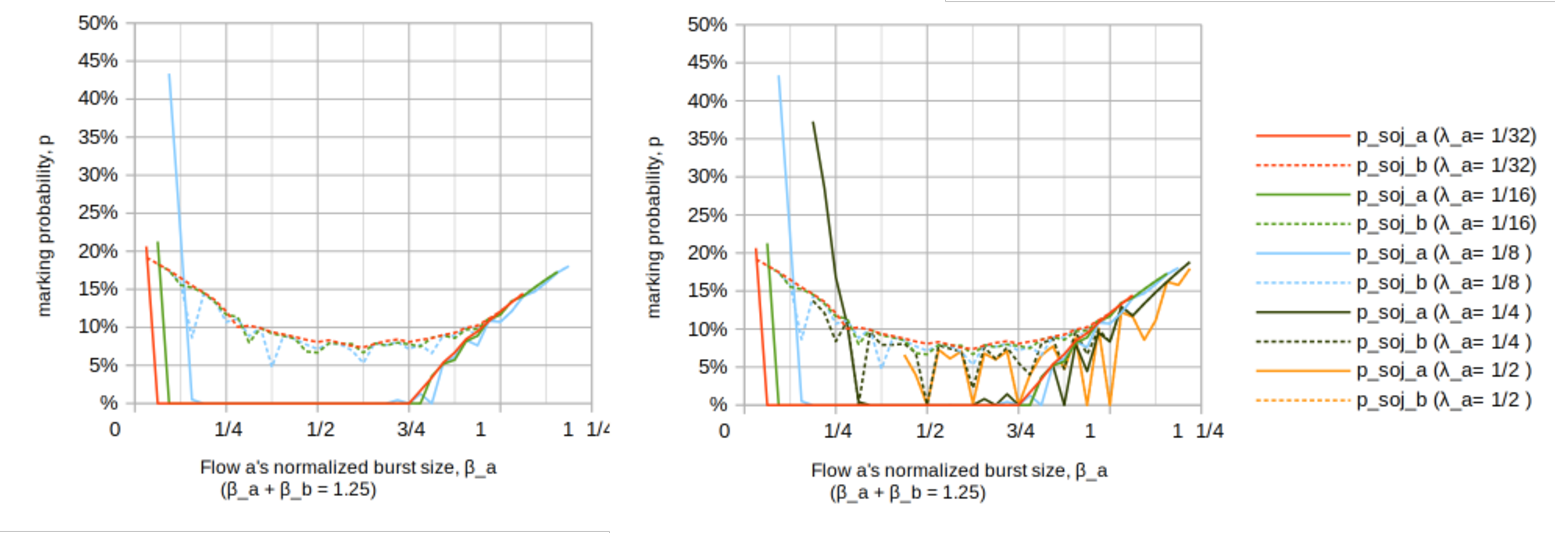
\includegraphics[width=\linewidth]{soj-fairnessSumBeta125}
	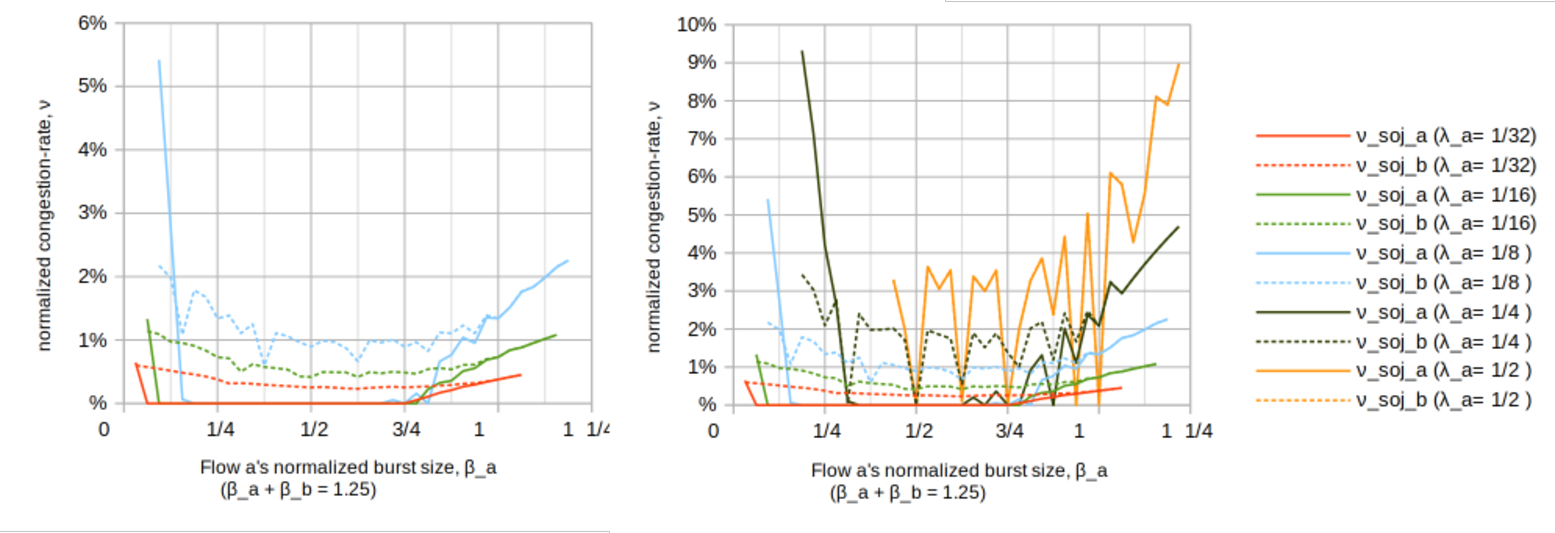
\includegraphics[width=\linewidth]{soj-cong-rateSumBeta125}
	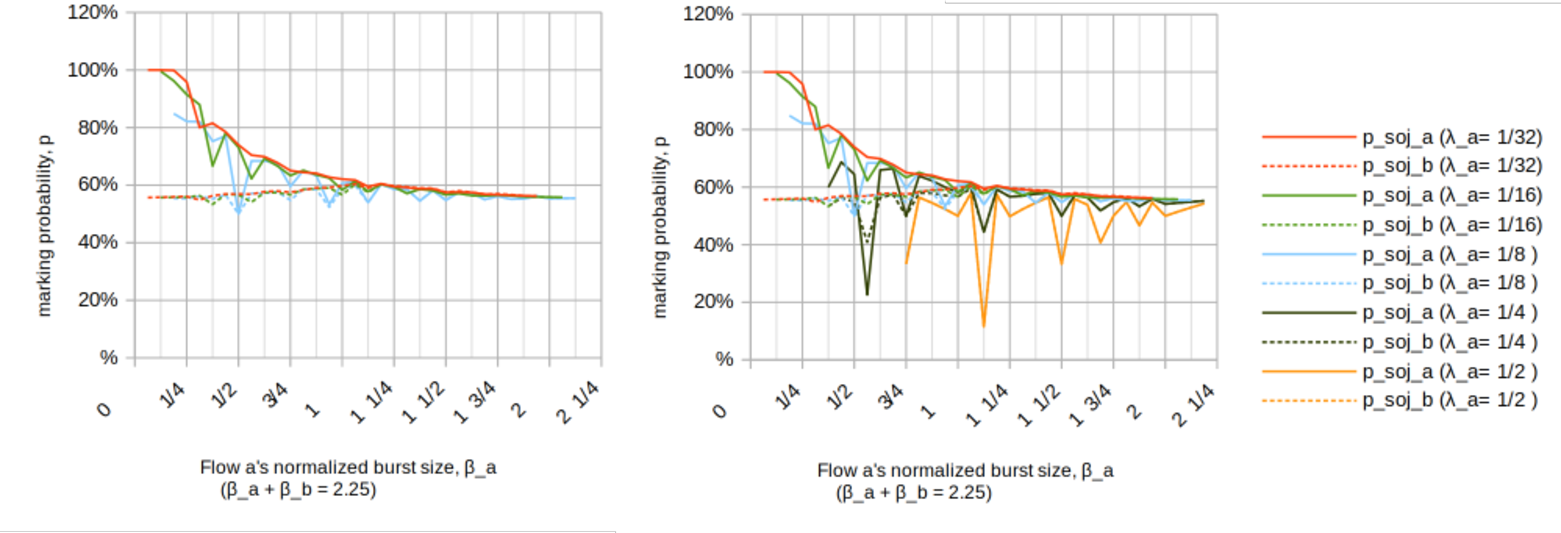
\includegraphics[width=\linewidth]{soj-fairnessSumBeta225}
	\caption{Sojourn-based marking fairness of two flows wrt capacity share, \(\lambda\), and relative burstiness, \(\beta\).\\
		\(\lambda_a+\lambda_b=100\%; \quad\mathrm{top:} \beta_a+\beta_b=1.0625;\) upper (marking prob) and lower (congestion-rate) middle: \(\beta_a+\beta_b=1.25 
		\quad\mathrm{bottom:} \beta_a+\beta_b=2.25\) (same as \autoref{fig:est-fairness-range}). 
}\label{fig:soj-fairness-range}
\end{figure*}

% ----------------------------------------------------------------
\subsection{Sojourn-based Marking Fairness}\label{sec:marking_fairness_expts_soj}

For comparison, \autoref{fig:soj-fairness-range} shows the ECN marking that results from sojourn-based marking under the same traffic scenarios as the EST-based marking in \autoref{fig:est-fairness-range} (note that the lower middle row is the same scenario as the upper middle, but the metric is normalized congestion-rate, which can be compared with \autoref{fig:cong-rate-range}).

The most obvious failing can be seen on the left-hand half of the lowest row (\(\beta_a+\beta_b=2.25\)), but also on the far-left of the other rows, where flow \(a\)'s marking exceeds \(b\)'s even though its burstiness and capacity share are both lower.
Similarly, on the right of the plots, no matter how bursty \(a\) becomes, its marking probability never exceeds \(b\)'s. Thus, sojourn-based marking sometimes perversely rewards burstiness and penalizes smoothness.

The second most obvious failing is the much lower overall marking probability in any of the scenarios, given the high degree of burstiness in all scenarios. Even when the bursts of flow \(a\) alone all exceed twice the marking threshold (\(\beta_a>2\) in the bottom row), marking is no higher than 60\% (in contrast, as  \(a\)'s bursts become smaller its marking perversely rises to 100\%). And in the middle case (\(\beta_a+\beta_b=2.25\)), even when all \(a\)'s bursts exceed the threshold (\(\beta_a>1\) the marking probability only lies in the 10\%--20\% range.

